\documentclass{beamer}

% \includeonlyframes{current}

\usepackage[T1]{fontenc}
\usepackage[utf8]{inputenc}
\usepackage[american]{babel}
\usepackage{amsmath,amsthm}
\usepackage{unicode}
\usepackage{ifthen}
\usepackage{tikz}
\usetikzlibrary{matrix,decorations,decorations.text,calc,arrows,snakes,shapes,positioning}

\usepackage[nosfdefault]{comicneue}
\usepackage{sourcesanspro}
\usepackage[amssymb,amsfonts]{concmath}
\usefonttheme[onlymath]{serif}
\usepackage{ulem}

\mode<presentation>{%
  \usetheme{Boadilla}
}
\beamertemplatenavigationsymbolsempty
\usecolortheme[RGB={110,0,124}]{structure}
\definecolor{title}{RGB}{110,0,124}
\setbeamercolor*{title}{fg=title}

\renewcommand{\emph}[1]{{\usebeamercolor[fg]{structure}#1}}

\newcommand{\C}{ℂ}
\newcommand{\R}{ℝ}
\newcommand{\Z}{ℤ}
\newcommand{\N}{ℕ}
\newcommand{\Q}{ℚ}
\newcommand{\F}{\mathbb{F}}
\renewcommand{\P}{\mathbb{P}}
\renewcommand{\O}{\mathcal{O}}
\newcommand{\tildO}{\mathcal{\tilde{O}}}
\newcommand{\poly}{\operatorname{poly}}
\newcommand{\polylog}{\operatorname{polylog}}
\newcommand{\End}{\operatorname{End}}
\newcommand{\Hom}{\operatorname{Hom}}
\newcommand{\Gal}{\operatorname{Gal}}
\newcommand{\chr}{\operatorname{char}}
\newcommand{\Cl}{\operatorname{Cl}}
\newcommand{\GL}{\operatorname{GL}}
\renewcommand{\a}{{\mathfrak{a}}}
\renewcommand{\b}{{\mathfrak{b}}}
\newcommand{\cyc}[1]{{〈 #1 〉}}
\newcommand{\ord}{\operatorname{ord}}
\newcommand{\mat}[1]{\left(\begin{smallmatrix}#1\end{smallmatrix}\right)}

\title[Maths of Isogeny Based Crypto]{Mathematics of Isogeny-based Cryptography}
\author{Luca De Feo}
\date[Birmingham IBC Workshop]{September 16, 2019\\
  Isogeny-based Cryptography Workshop\\
  Birmingham\\
  \medskip
  Slides online at \textcolor{blue}{\url{https://defeo.lu/docet}}}
\institute[IBM Research]{IBM Research, Zürich}

\begin{document}

\frame[plain]{\titlepage}

%%

\begin{frame}{Projective space}
  \begin{definition}[Projective space]
    Let $\bar{k}$ an algebraically closed field, the \emph{projective
      space} $\P^n(\bar{k})$ is the set of non-null $(n+1)$-tuples
    $(x_0,\dots,x_n)\in \bar{k}^n$ modulo the equivalence relation
    \[(x_0,\dots,x_n) \sim (\lambda x_0, \dots, \lambda x_n) \qquad
      \text{with $\lambda\in \bar{k}\setminus\{0\}$}.\]
    A class is denoted by $(x_0:\cdots:x_n)$.
  \end{definition}

  \centering
  \includegraphics[height=0.5\textheight]{camera-obscura.jpg}
\end{frame}

%%

\begin{frame}{Weierstrass equations}
  \begin{columns}
    \begin{column}{0.4\textwidth}
      Let $k$ be a field of characteristic $\ne 2,3$.

      An \emph{elliptic curve \textit{defined over $k$}} is the locus
      in $\P^2(\bar{k})$ of an equation
      \[\emph{Y^2Z = X^3 + aXZ^2 + bZ^3},\]
      where $a,b\in k$ and $4a^3+27b^2\ne 0$.

      \begin{itemize}
      \item<2-> $\O=(0:1:0)$ is the \emph{point at infinity};
      \item<3-> $y^2 = x^3 + ax + b$ is the \emph{affine equation}.
      \end{itemize}
    \end{column}
    \begin{column}{0.6\textwidth}
      \begin{center}
        \begin{tikzpicture}[domain=-2.4566:4,samples=100,yscale=1/2]
          \draw plot (\x,{sqrt(\x*\x*\x-4*\x+5)});
          \draw plot (\x,{-sqrt(\x*\x*\x-4*\x+5)});

          \draw[thin,gray,-latex] (0,-7) -- (0,7);
          \draw[thin,gray,-latex] (-3,0) -- (4,0);
        \end{tikzpicture}
      \end{center}
    \end{column}
  \end{columns}
\end{frame}

%%

\begin{frame}{Attention: arithmetic geometry!}
  \begin{columns}
    \begin{column}{0.55\textwidth}
      \[\emph{E \;:\; y^2 = x^3 - 2x + 1}\]

      \bigskip
      
      \emph{Rational} points:
      \begin{itemize}
      \item<1-> $\emph{E(ℚ)} = \{ (1,0), (0,1), (0,-1), \O \}$,
      \item<2-> $\emph{\#E(ℚ(\sqrt{5}))} = 8$,
      \item<3-> \dots
      \item<3-> $\emph{\#E(ℝ)} = ∞$.
      \item<4-> $\emph{\#E(ℂ)} = ∞$.
      \end{itemize}
    \end{column}
    \begin{column}{0.45\textwidth}
      \begin{center}
        \begin{tikzpicture}
          \draw[thin,gray,-latex] (0,-4) -- (0,4);
          \draw[thin,gray,-latex] (-2,0) -- (3,0);

          \draw[fill] (1,0) circle (1pt) (0,1) circle (1pt) (0,-1) circle (1pt);
          \uncover<2->{
            \draw[fill] (-1.61803,0) circle (1pt) (0.61803,0) circle (1pt)
            (2,2.23606) circle (1pt) (2,-2.23606) circle (1pt);
          }

          \begin{uncoverenv}<3->
            \begin{scope}
              [domain=-1.61803:0.61803,samples=50]
              \draw plot (\x,{sqrt(\x*\x*\x-2*\x+1)});
              \draw plot (\x,{-sqrt(\x*\x*\x-2*\x+1)});
            \end{scope}
            \begin{scope}
              [domain=1:2.5,samples=50]
              \draw plot (\x,{sqrt(\x*\x*\x-2*\x+1)});
              \draw plot (\x,{-sqrt(\x*\x*\x-2*\x+1)});
            \end{scope}
          \end{uncoverenv}          
        \end{tikzpicture}
      \end{center}
    \end{column}
  \end{columns}  
\end{frame}

%%

\begin{frame}{The group law}
  \begin{columns}
    \begin{column}{0.4\textwidth}
      \begin{block}{Bezout's theorem}
        Every line cuts $E$ in exactly three points (counted with
        multiplicity).
      \end{block}

      Define a \emph{group law} such that any three colinear points
      add up to zero.

      \begin{itemize}
      \item<2-> The law is \emph{algebraic}\\ (it has \textit{formulas});
      \item<3-> The law is \emph{commutative};
      \item<3-> $\O$ is the \emph{group identity};
      \item<3-> \emph{Opposite points} have the same $x$-value.
      \end{itemize}
    \end{column}
    \begin{column}{0.6\textwidth}
      \begin{center}
        \begin{tikzpicture}[domain=-2.4566:4,samples=100,yscale=1/2]
          \draw plot (\x,{sqrt(\x*\x*\x-4*\x+5)});
          \draw plot (\x,{-sqrt(\x*\x*\x-4*\x+5)});

          \draw[thin,gray,-latex] (0,-7) -- (0,7);
          \draw[thin,gray,-latex] (-3,0) -- (4,0);
          \draw (-3,1) -- (4,8/3+3);
          \begin{scope}[every node/.style={draw,circle,inner sep=1pt,fill},cm={1,2/3,0,0,(0,3)}]
            \node at (-2.287980,0) {};
            \node at (-0.535051,0) {};
            \node at (3.267475,0) {};
          \end{scope}
          \begin{scope}[every node/.style={yshift=0.3cm},cm={1,2/3,0,0,(0,3)}]
            \node at (-2.287980,0) {$P$};
            \node at (-0.535051,0) {$Q$};
            \node at (3.267475,0) {$R$};
          \end{scope}

          \draw[dashed] (3.267475,3.267475*2/3+3) -- (3.267475,-3.267475*2/3-3) 
          node[draw,circle,inner sep=1pt,fill] {}
          node[xshift=-0.1cm,anchor=east] {$P+Q$};
        \end{tikzpicture}
      \end{center}
    \end{column}
  \end{columns}
\end{frame}

%%

\begin{frame}{What are elliptic curves?}
  \begin{block}{For mathematicians}
    \begin{itemize}
    \item The \emph{smooth projective curves of genus 1} (with a
      distinguished point);
    \item The simplest \emph{abelian varieties} (dimension 1);
    \item Finitely generated abelian groups of mysterious free rank
      (aka \emph{BSD conjecture});
    \item What you use to make examples.
    \end{itemize}
  \end{block}

  \pause
  
  \begin{block}{For cryptographers}
    \begin{itemize}
    \item \emph{Finite abelian} groups (often cyclic);
    \item Easy to compute the order;
    \item ``2-dimensional'' generalizations of $μ_k$ (the \emph{roots
        of unity} of $k$)\dots
    \item \dots with \emph{bilinear maps} (aka \emph{pairings})!
    \end{itemize}
  \end{block}
\end{frame}

%%

\begin{frame}{Maps: isomorphisms}
  \begin{block}{Isomorphisms}
    The only \emph{invertible algebraic maps} between elliptic curves
    are of the form
    \[(x,y) \mapsto (u^2x, u^3y)\]
    for some $u\in\bar{k}$.

    They are \emph{group isomorphisms}.
  \end{block}

  \begin{block}{$j$-Invariant}
    Let $E\;:\;y^2=x^3+ax+b$, its \emph{$j$-invariant} is
    \[j(E) = 1728\frac{4a^3}{4a^3+27b^2}.\]

    Two elliptic curves $E,E'$ are \emph{isomorphic} if and only if
    $j(E)=j(E')$.
  \end{block}
\end{frame}

%%

\begin{frame}{Group structure}
  \begin{block}{Torsion structure}
    Let $E$ be defined over an algebraically closed field $\bar{k}$ of
    characteristic $p$.
    \begin{align*}
      E[m] \simeq\quad& \Z/m\Z\times\Z/m\Z  &\text{if $p\nmid m$,}\\[1em]
                 &\Z/p^e\Z & \text{\emph{ordinary} case,}\\[-1.7em]
      E[p^e] \simeq\Biggl\{& \\[-1.7em]
                 &\{\O\} & \text{\emph{supersingular} case.}
    \end{align*}
  \end{block}

  \begin{block}{Finite fields (Hasse's theorem)}
    Let \emph{$E$} be defined over a finite field \emph{$\F_q$}, then
    \[\lvert\#E(\F_q) - q - 1\rvert \le 2\sqrt{q}.\]
    In particular, there exist integers \emph{$n_1$} and
    \emph{$n_2|\gcd(n_1,q-1)$} such that
    \[E(\F_q) ≃ ℤ/n_1ℤ × ℤ/n_2ℤ.\]
  \end{block}
\end{frame}

%%

\begin{frame}
  \frametitle{Maps: what's \alt<2->{\xout{scalar multiplication} an
      isogeny}{scalar multiplication}?}

  \begin{overlayarea}{\textwidth}{4em}
    \Large
    \[
      \alt<3->{\phi}{[n]}
      \;:\; P \mapsto
      \alt<3->{\phi(P)}{\underbrace{P + P + \cdots + P}_{n\text{ times}}}\]
  \end{overlayarea}
  
  \begin{itemize}
  \item A map \emph{$E\to \alt<4->{\xout{E} E'}{E\phantom{\xout{}}}$},
  \item a \emph{group morphism},
  \item with \emph{finite kernel}\\
    \alt<5->{(\xout{the torsion group $E[n]\simeq(ℤ/nℤ)^2$} any
      finite subgroup \emph{$H\subset E$})}{(the torsion group
      \emph{$E[n]\simeq(ℤ/nℤ)^2$})},
  \item \emph{surjective} (in the algebraic closure),
  \item given by \emph{rational maps} of degree \alt<6->{\xout{$n^2$}
      \emph{$\#H$}}{\emph{$n^2$}}.
  \end{itemize}

  \medskip
  
  \begin{uncoverenv}<7->
    (Separable) isogenies $\Leftrightarrow$ finite subgroups:
    \alert{\[0 \to H \to E \overset{\phi}{\to} E' \to 0\]}
  \end{uncoverenv}
\end{frame}

%% 

\begin{frame}{Isogenies: an example over $\F_{11}$}
  \begin{tikzpicture}[scale=0.4]
    \begin{scope}
      \node[anchor=center] at (0,7) {$E \;:\; y^2 = x^3 + x$};

      \uncover<-1>{
        \draw[thin,gray] (0,-6) -- (0,6);
        \draw[thin,gray] (-6,0) -- (6,0);
      }

      \foreach \x/\y in {0/0,5/3,-4/3,-3/5,-2/1,-1/3} {
        \draw[blue,fill] (\x,\y) circle (0.2) node(E_\x_\y){}
        (\x,-\y) circle (0.2) node(E_\x_-\y){};
      }

      \uncover<2->{\draw[red,fill] (0,0) circle (0.3);}
    \end{scope}

    \draw[black!10!white,thick] (8,-7) -- +(0,14);
    
    \begin{scope}[shift={(16,0)}]
      \node at (0,7) {$E' \;:\; y^2 = x^3 - 4x$};

      \uncover<-1>{
        \draw[thin,gray] (0,-6) -- (0,6);
        \draw[thin,gray] (-6,0) -- (6,0);
      }

      \foreach \x/\y in {0/0,2/0,3/2,4/2,6/4,-2/0,-1/5} {
        \draw[color=blue,fill] (\x,\y) circle (0.2) node(F_\x_\y){}
        (\x,-\y) circle (0.2) node(F_\x_-\y){};
      }
    \end{scope}

    \begin{scope}[color=red,-latex,dashed]
      \begin{uncoverenv}<2->
        \path
        (E_5_3) edge (F_3_2)
        (E_-4_3) edge (F_4_-2)
        (E_-3_5) edge (F_4_2)
        (E_-2_1) edge (F_3_-2)
        (E_-1_3) edge (F_-2_0);
      \end{uncoverenv}
      \begin{uncoverenv}<2->
        \path
        (E_5_-3) edge (F_3_-2)
        (E_-4_-3) edge (F_4_2)
        (E_-3_-5) edge (F_4_-2)
        (E_-2_-1) edge (F_3_2)
        (E_-1_-3) edge (F_-2_0);
      \end{uncoverenv}
    \end{scope}
  \end{tikzpicture}
  
  \begin{columns}
    \begin{column}{0.5\textwidth}
      \[\phi(x,y) = \left(\frac{x^2 + 1}{x},\quad y\frac{x^2-1}{x^2}\right)\]
    \end{column}
    \begin{column}{0.5\textwidth}
      \begin{itemize}
      \item<2-> Kernel generator in \alert{red}.
      \item<2-> This is a degree $2$ map.
      \item<2-> Analogous to $x\mapsto x^2$ in $\F_q^*$.
      \end{itemize}
    \end{column}
  \end{columns}
\end{frame}

%%

\begin{frame}{Maps: isogenies}
  \begin{theorem}
    Let $\phi:E\to E'$ be a map between elliptic curves. These
    conditions are equivalent:
    \begin{itemize}
    \item $\phi$ is a \emph{surjective group morphism},
    \item $\phi$ is a \emph{group morphism} with \emph{finite kernel},
    \item $\phi$ is a non-constant \emph{algebraic map} of projective
      varieties sending the point at infinity of $E$ onto the point at
      infinity of $E'$.
    \end{itemize}
    If they hold $\phi$ is called an \emph{isogeny}.
  \end{theorem}

  Two curves are called \emph{isogenous} if there exists an isogeny
  between them.

  \begin{block}{Example: Multiplication-by-$m$}
    On any curve, an isogeny from $E$ to itself (i.e., an
    \emph{endomorphism}):
    \begin{align*}
      [m] \;:\; E &\to E,\\
      P &\mapsto [m]P.
    \end{align*}
  \end{block}
\end{frame}

%%

\begin{frame}{Isogeny lexicon}
  \begin{block}{Degree}
    \begin{itemize}
    \item $\approx$ degree of the rational fractions defining the isogeny;
    \item Rough measure of the information needed to encode it.
    \end{itemize}
  \end{block}
  
  \begin{block}{Separable, inseparable, cyclic}
    An isogeny $ϕ$ is \emph{separable} iff \emph{$\degϕ=\#\kerϕ$}.

    \begin{itemize}
    \item Given \emph{$H⊂E$} finite, write \emph{$ϕ : E → E/H$} for
      the \emph{unique} separable isogeny s.t. \emph{$\kerϕ=H$}.
    \item $ϕ$ \emph{inseparable} $⇒$ $p$ divides $\degϕ$.
    \item \emph{Cyclic isogeny} $≡$ separable isogeny with cyclic
      kernel.
      \begin{itemize}
      \item \emph{Non-example:} the multiplication map $[m]:E→E$.
      \end{itemize}
    \end{itemize}
  \end{block}

  \begin{block}{Rationality}
    Given $E$ \emph{defined over $k$}, an isogeny $ϕ$ is rational if
    $\ker ϕ$ is \emph{Galois invariant}.
    \begin{itemize}
    \item[$⇒$] $ϕ$ is represented by rational fractions with
      coefficients in $k$.
    \end{itemize}
  \end{block}
\end{frame}

%%

\begin{frame}{The dual isogeny}
  Let $\phi:E\to E'$ be an isogeny of degree $m$. 
  There is a unique isogeny $\hat{\phi}:E'\to E$ such that
  \[\hat{\phi}\circ\phi = [m]_E, \quad \phi\circ\hat{\phi} = [m]_{E'}.\]
  $\hat{\phi}$ is called the \emph{dual isogeny of $\phi$}; it has the
  following properties:
  
  \begin{enumerate}
  \item $\hat{\phi}$ is defined over $k$ if and only if $\phi$ is;
  \item $\widehat{\psi\circ\phi} = \hat{\phi}\circ\hat{\psi}$ for any isogeny $\psi:E'\to E''$;
  \item $\widehat{\psi+\phi} = \hat{\psi} + \hat{\phi}$ for any isogeny $\psi:E\to E'$;
  \item $\deg \phi = \deg\hat{\phi}$;
  \item $\hat{\hat{\phi}} = \phi$.
  \end{enumerate}
\end{frame}

%%

\begin{frame}{Up to \emph{isomorphism}}
  \begin{center}
    \begin{tikzpicture}[domain=-2.4566:4,samples=100]
      \newcount\zoomout
      \transduration<15-21>{0.5}
      \animatevalue<15-20>{\zoomout}{0}{10}
      \begin{uncoverenv}<-20>
        \begin{scope}[scale=1-0.09*\zoomout]
          \begin{scope}
            \draw[thin,gray,-latex] (0,-4) -- (0,4);
            \draw[thin,gray,-latex] (-4.2,0) -- (7,0);
          \end{scope}
          
          \newcount\xstretch
          \newcount\ystretch
          \newcount\slant
          \transduration<1-13>{0.5}
          \animatevalue<1-5>{\xstretch}{0}{4}
          \animatevalue<5-9>{\ystretch}{0}{4}
          \animatevalue<9-13>{\slant}{0}{4}      
          \begin{scope}[yscale=0.55-0.05*\the\ystretch,xscale=1+0.1*\the\xstretch,xslant=0.02*\slant]
            \draw plot (\x,{sqrt(\x*\x*\x-4*\x+5)});
            \draw plot (\x,{-sqrt(\x*\x*\x-4*\x+5)});

            \begin{uncoverenv}<-18>
              \draw (-3,1) -- (4,8/3+3);
              \begin{scope}[every node/.style={draw,circle,inner sep=1pt,fill},cm={1,2/3,0,0,(0,3)}]
                \node at (-2.287980,0) {};
                \node at (-0.535051,0) {};
                \node at (3.267475,0) {};
              \end{scope}
              \begin{scope}[every node/.style={yshift=0.3cm},cm={1,2/3,0,0,(0,3)}]
                \node at (-2.287980,0) {$P$};
                \node at (-0.535051,0) {$Q$};
                \node at (3.267475,0) {$R$};
              \end{scope}
              \draw[dashed] (3.267475,3.267475*2/3+3) -- (3.267475,-3.267475*2/3-3) 
              node[draw,circle,inner sep=1pt,fill] {}
              node[xshift=-0.1cm,anchor=east] {$P+Q$};
            \end{uncoverenv}
          \end{scope}

          \begin{uncoverenv}<14>
            \node[anchor=west] at (-4,-3) {\Large\alert{$y^2=x^3+ax+b \quad\longrightarrow\quad j\equiv 1728\frac{4a^3}{4a^3+27b^2}$}};
          \end{uncoverenv}
        \end{scope}
      \end{uncoverenv}
      
      \begin{uncoverenv}<21->
        \draw[fill] (0,0) circle (2pt) node[anchor=north] {$j=1728$};
        \uncover<22>{
          \draw (0.1,0) edge[bend left,->] node[auto] {$\phi$} (7,0);
        }
        \uncover<22->{
          \draw[fill] (7.1,0) circle (2pt) node[anchor=north] {$j=287496$};
        }
        \uncover<23->{
          \draw (0.1,0) edge[bend left,<->,red,very thick] (7,0);
        }
      \end{uncoverenv}
    \end{tikzpicture}
  \end{center}  
\end{frame}

%%

\begin{frame}{Isogeny graphs}
  \begin{block}{Serre-Tate theorem}
    Two elliptic curves $E,E'$ defined over a finite field $\F_q$ are
    \emph{isogenous}\\
    (over $\F_q$) iff \emph{$\#E(\F_q) = \#E'(\F_q)$}.
  \end{block}

  \smallskip

  \begin{columns}
    \begin{column}{0.5\textwidth}
      \emph{Isogeny graphs}
      \begin{itemize}
      \item \emph{Vertices are curves} up to isomorphism,
      \item \emph{Edges are isogenies} up to isomorphism.
      \end{itemize}

      \emph{Isogeny volcanoes}
      \begin{itemize}
      \item Curves are ordinary,
      \item Isogenies all have degree a prime $\ell$.
      \end{itemize}
    \end{column}      
    \begin{column}{0.5\textwidth}
      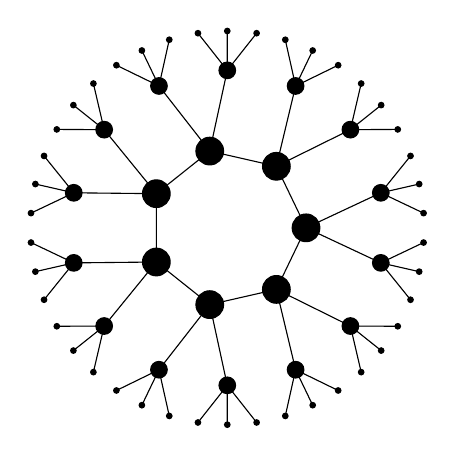
\begin{tikzpicture}
        \begin{scope}
          \def\crater{7}
          \foreach \i in {1,...,\crater} {
            \draw[fill] (360/\crater*\i:1cm) circle (5pt);
            \draw (360/\crater*\i : 1cm) -- (360/\crater*\i+360/\crater : 1cm);
            \foreach \j in {-1,1} {
              \draw[fill] (360/\crater*\i : 1cm) -- (360/\crater*\i + \j*360/\crater/4 : 2cm) circle (3pt);
              \foreach \k in {-1,0,1} {
                \draw[fill] (360/\crater*\i + \j*360/\crater/4 : 2cm) --
                (360/\crater*\i + + \j*360/\crater/4 + \k*360/\crater/6 : 2.5cm) circle (1pt);
              }
            }
          }
        \end{scope}
      \end{tikzpicture}
    \end{column}
  \end{columns}
\end{frame}

%%

\begin{frame}{What do isogeny graphs look like?}
  \begin{columns}
    \begin{column}{0.46\textwidth}
      \begin{block}{Torsion subgroups ($ℓ$ prime)}
        In an algebraically closed field:
        \[\emph{E[ℓ] = 〈P,Q〉 ≃ (ℤ/ℓℤ)^2}\]
        \[\Downarrow\]
        There are exactly \emph{$ℓ+1$} cyclic subgroups \emph{$H⊂E$}
        of order $ℓ$:
        \[\emph{〈P+Q〉, 〈P+2Q〉, \dots, 〈P〉, 〈Q〉}\]
        \[\Downarrow\]
        There are exactly \emph{$ℓ+1$} distinct isogenies of degree
        \emph{$ℓ$}.
      \end{block}
    \end{column}
    \begin{column}{0.54\textwidth}
      \centering
      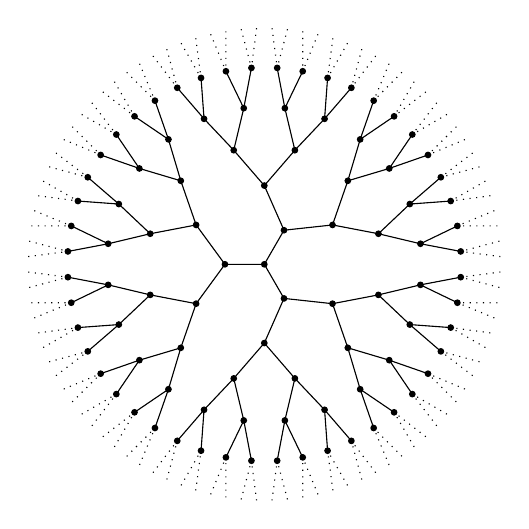
\begin{tikzpicture}[scale=0.5]
        \def\levels{6}
        \draw[fill] (0:0) circle (2pt);
        \foreach \i in {1,...,\levels} {
          \pgfmathparse{3*2^\i}
          \let\nodes\pgfmathresult
          \foreach \j in {1,3,...,\nodes} {
            \pgfmathparse{\j + (-1)^div(\j,2)}
            \let\lower\pgfmathresult
            \ifthenelse{\i = \levels}{
              \draw[dotted] (360/\nodes*\j : \i) --
              (360/\nodes*\lower : \i - 1);
            }{
              \draw[fill] (360/\nodes*\j : \i) circle (2pt) --
              (360/\nodes*\lower : \i - 1);
            }
          }
        }
      \end{tikzpicture}
      (non-CM) $2$-isogeny graph over $ℂ$
    \end{column}
  \end{columns}
\end{frame}  
  
%%

\begin{frame}{What happens over a finite field $\F_p$?}
  \begin{block}{Rational isogenies ($ℓ≠p$)}
    In the algebraic closure \emph{$\bar{\F}_p$}
    \[\emph{E[ℓ] = 〈P,Q〉 ≃ (ℤ/ℓℤ)^2}\]
    However, an isogeny is \emph{defined over $\F_p$} only if its kernel
    is \emph{Galois invariant}.
  \end{block}

  \begin{columns}
    \begin{column}{0.47\textwidth}
      Enter the \emph{Frobenius map}
      \begin{align*}
        π : E &→ E\\
        (x,y) &↦ (x^p,y^p)
      \end{align*}
      \emph{$E$} is seen here as a curve over \emph{$\bar{\F}_p$}.
    \end{column}
    \begin{column}{0.47\textwidth}
      \begin{block}{The Frobenius action on $E[ℓ]$}
        \transduration<2-5>{0.5}
        \transdissolve<2-5>
        \begin{tikzpicture}[]
          \uncover<1>{
            \node at (0,0){$π(P) =$};   
            \node at (0,-0.7){$π(Q) =$};
          }
          \node at (1.8,0){$a\uncover<-3>{P +} b\uncover<-3>{Q}$};
          \node at (1.8,-0.7){$c\uncover<-3>{P +} d\uncover<-3>{Q}$};
          \uncover<3->{
            \node at (0.8,-0.35){$\Biggl($}; \node at (2.7,-0.35){$\Biggr)$};
          }
          \uncover<5->{
            \node at (0.3,-0.35){$π:$};
            \node at (3.3,-0.35){$\mod ℓ$};
          }
        \end{tikzpicture}

        \uncover<6->{We identify \emph{$π|E[ℓ]$} to a conjugacy class
          in \emph{$\GL(ℤ/ℓℤ)$}.}
      \end{block}
    \end{column}
  \end{columns}
\end{frame}

%%

\begin{frame}{What happens over a finite field $\F_p$?}
  \begin{center}
    Galois invariant proper subgroups of \emph{$E[ℓ]$}\\
    =\\
    eigenspaces of \emph{$π∈\GL(ℤ/ℓℤ)$}\\
    =\\
    rational isogenies of \emph{degree $ℓ$}
  \end{center}
  \pause
  \begin{block}{How many Galois invariant subgroups?}
    \begin{itemize}
    \item \emph{$π|E[ℓ] \sim \mat{λ&0\\0&λ}$}
      \hfill $→ \emph{ℓ+1}$ isogenies
    \item \emph{$π|E[ℓ] \sim \mat{λ&0\\0&μ}$} with \emph{$λ≠μ$}
      \hfill $→$ \emph{two} isogenies
    \item \emph{$π|E[ℓ] \sim \mat{λ&*\\0&λ}$}
      \hfill $→$ \emph{one} isogeny
    \item \emph{$π|E[ℓ]$} has no eigenvalues in \emph{$ℤ/ℓℤ$}
      \hfill $→$ \emph{no} isogeny
    \end{itemize}
  \end{block}
\end{frame}

%%

\begin{frame}{Algebras, orders}
  \begin{itemize}
  \item A \emph{quadratic imaginary number field} is an extension of
    $\Q$ of the form $Q[\sqrt{-D}]$ for some non-square $D>0$.
  \item A \emph{quaternion algebra} is an algebra of the form
    $\Q + \alpha\Q + \beta\Q + \alpha\beta\Q$, where the generators
    satisfy the relations
    \[\alpha^2,\beta^2\in\Q, \quad \alpha^2<0, \quad \beta^2 < 0, \quad \beta\alpha=-\alpha\beta.\]
  \end{itemize}
  
  \begin{block}{Orders}
    Let $K$ be a finitely generated $\Q$-algebra.  An \emph{order}
    $\O\subset K$ is a \emph{subring} of $K$ that is a finitely
    generated $\Z$-module of \emph{maximal dimension}.  An order that
    is not contained in any other order of $K$ is called a
    \emph{maximal order}.
  \end{block}

  Examples:
  \begin{itemize}
  \item $\Z$ is the only order contained in $\Q$,
  \item $\Z[i]$ is the only maximal order of $\Q(i)$,
  \item $\Z[\sqrt{5}]$ is a non-maximal order of $\Q(\sqrt{5})$,
  \item The \emph{ring of integers} of a number field is its only
    maximal order,
  \item In general, maximal orders in quaternion algebras are
    \emph{not unique}.
  \end{itemize}
\end{frame}

\begin{frame}{The endomorphism ring}
  The \emph{endomorphism ring} $\End(E)$ of an elliptic curve $E$ is
  the ring of all isogenies $E\to E$ (plus the null map) with
  \emph{addition} and \emph{composition}.

  \begin{block}{Theorem (Deuring)}
    Let $E$ be an elliptic curve defined over a field $k$ of
    characteristic $p$.\\
    $\End(E)$ is isomorphic to one of the following:
    \begin{itemize}
    \item $\Z$, only if $p=0$
      \begin{flushright}
        $E$ is \emph{ordinary}.
      \end{flushright}
    \item An order $\O$ in a quadratic imaginary field:
      \begin{flushright}
        $E$ is \emph{ordinary} with \emph{complex multiplication} by
        $\O$.
      \end{flushright}
    \item Only if $p>0$, a maximal order in a quaternion
      algebra\footnote{(ramified at $p$ and $\infty$)}:
      \begin{flushright}
        $E$ is \emph{supersingular}.
      \end{flushright}
    \end{itemize}
  \end{block}
\end{frame}

%%

\begin{frame}{The finite field case}
  \begin{block}{Theorem (Hasse)}
    Let $E$ be defined over a finite field. Its Frobenius endomorphism
    $\pi$ satisfies a quadratic equation
    \[\pi^2 - t\pi + q = 0\]
    in $\End(E)$ for some $|t|\le2\sqrt{q}$, called the \emph{trace}
    of $\pi$.  The trace $t$ is coprime to $q$ if and only if $E$ is
    ordinary.
  \end{block}

  Suppose $E$ is \emph{ordinary}, then $D_\pi=t^2-4q<0$ is the
  \emph{discriminant} of $\Z[\pi]$.
  
  \begin{itemize}
  \item $K=\Q(\pi)=\Q(\sqrt{D_\pi})$ is the \emph{endomorphism algebra} of $E$.
  \item Denote by $\O_K$ its ring of integers, then
    \[\Z \ne \Z[\pi] \subset \End(E) \subset \O_K.\]
  \end{itemize}

  In the \emph{supersingular} case, $\pi$ may or may not be in $\Z$,
  depending on $q$.
\end{frame}

%%

\begin{frame}{Endomorphism rings of ordinary curves}
  \begin{block}{Classifying quadratic orders}
    Let $K$ be a quadratic number field, and let $\O_K$ be its ring of
    integers.
    \begin{itemize}
    \item Any order $\O\subset K$ can be written as $\O=\Z+f\O_K$ for
      an integer $f$, called the \emph{conductor} of $\O$, denoted by
      $[\O_k:\O]$.
    \item If $d_K$ is the \emph{discriminant} of $K$, the discriminant
      of $\O$ is $f^2d_K$.
    \item If $\O,\O'$ are two orders with discriminants $d,d'$, then
      \emph{$\O\subset\O'$ iff $d'|d$}.
    \end{itemize}
  \end{block}

  \bigskip
  
  \centering
  \begin{tikzpicture}[xscale=3,yscale=1.1]
    \node(OK) at (0,0) {$\O_K$};
    \node(O2) at (-1,-1) {$\Z+2\O_K$};
    \node(O3) at (0,-1) {$\Z+3\O_K$};
    \node(O5) at (1,-1) {$\Z+5\O_K$};
    \node(O6) at (-1,-2) {$\Z+6\O_K$};
    \node(O10) at (0,-2) {$\Z+10\O_K$};
    \node(O15) at (1,-2) {$\Z+15\O_K$};
    \node(O30) at (0,-3) {$\Z[\pi]\simeq\Z+30\O_K$};

    \begin{scope}
      \draw
      (OK) edge (O2) edge (O3) edge (O5)
      (O2) edge (O6) edge (O10)
      (O3) edge (O6) edge (O15)
      (O5) edge (O10) edge (O15)
      (O30) edge (O6) edge (O15) edge (O10);
    \end{scope}
  \end{tikzpicture}
\end{frame}

%%

\begin{frame}{Volcanology (Kohel 1996)}

  \begin{columns}
    \begin{column}{0.5\textwidth}
      Let \emph{$E,E'$} be curves with respective endomorphism rings \emph{$\O,\O'⊂K$}.\\
      Let \emph{$ϕ:E→E'$} be an isogeny of prime degree \emph{$ℓ$},
      then:
    \end{column}
    \begin{column}{0.5\textwidth}
      \centering{}
      \begin{tabular}{l l}
        if $\O=\O'$, & $ϕ$ is \emph{horizontal};\\
        if $[\O':\O]=ℓ$, & $ϕ$ is \emph{ascending};\\
        if $[\O:\O']=ℓ$, & $ϕ$ is \emph{descending}.
      \end{tabular}      
    \end{column}
  \end{columns}

  \bigskip

  \centering
  \begin{tikzpicture}
    \def\crater{7}
    \foreach \i in {1,...,\crater} {
      \draw[fill] (360/\crater*\i:1cm) circle (5pt);
      \draw (360/\crater*\i : 1cm) -- (360/\crater*\i+360/\crater : 1cm);
      \foreach \j in {-1,1} {
        \draw[fill] (360/\crater*\i : 1cm) -- (360/\crater*\i + \j*360/\crater/4 : 2cm) circle (3pt);
        \foreach \k in {-1,0,1} {
          \draw[fill] (360/\crater*\i + \j*360/\crater/4 : 2cm) --
          (360/\crater*\i + + \j*360/\crater/4 + \k*360/\crater/6 : 2.5cm) circle (1pt);
        }
      }
    }
    \begin{scope}[xshift=4cm]
      \node at (0,2) {$\End(E)$};
      \draw[fill] (0,1) circle(5pt) node[xshift=0.7cm]{$\O_K$} -- 
      (0,0) circle(3pt) --
      (0,-1) circle(1pt) node[xshift=0.7cm]{$ℤ[π]$};
    \end{scope}
  \end{tikzpicture}
  
  \small
  Ordinary isogeny volcano of degree $ℓ=3$.
\end{frame}

%%

\begin{frame}{Volcanology (Kohel 1996)}
  \centering
  \begin{columns}
    \begin{column}{0.35\textwidth}
      Let $E$ be ordinary, \emph{$\End(E)⊂K$}.

      \bigskip

      $\O_K$: \emph{maximal order} of $K$,\\
      $D_K$: \emph{discriminant} of $K$.

      \bigskip
      
      \uncover<2->{Height \emph{$= v_ℓ([\O_K:ℤ[π]])$}.}
      
      \bigskip
      
      \uncover<3->{\alert{How large is the crater?}}
    \end{column}
    \begin{column}{0.65\textwidth}
      \centering
      \begin{tikzpicture}[scale=0.8]
        \small
        \begin{scope}
          \draw[fill] (0,0) circle (2pt)
          -- (-1,-1) circle (2pt)
          (0,0) -- (0,-1) circle (2pt)
          (0,0) -- (1,-1) circle (2pt);
          \node at (0,-2) {$\left(\frac{D_K}{ℓ}\right) = -1$};
        \end{scope}    

        \begin{scope}[xshift=3.5cm]
          \draw[fill] (0,0) circle (2pt)
          -- (-0.5,-1) circle (2pt)
          (0,0) -- (0.5,-1) circle (2pt)
          (0,0) -- (2,0) circle (2pt)
          -- (1.5,-1) circle (2pt)
          (2,0) -- (2.5,-1) circle (2pt);
          \node at (1,-2) {$\left(\frac{D_K}{ℓ}\right) = 0$};
        \end{scope}
        
        \begin{scope}[xshift=2.5cm,yshift=-3cm]
          \draw[fill] (-0.8,0) node[coordinate] (A) {} circle (2pt)
          -- +(0,-1) circle (2pt)
          (0,-0.3) node[coordinate] (B) {} circle (2pt)
          -- +(0,-1) circle (2pt)
          (0.8,0) node[coordinate] (C) {} circle (2pt)
          -- +(0,-1) circle (2pt);
          \draw[bend right=20]
          (A) edge (B)
          (B) edge (C)
          (C) edge[dashed,bend right=90] (A);
          \node at (0,-2) {$\left(\frac{D_K}{ℓ}\right) = +1$};
        \end{scope}
      \end{tikzpicture}
    \end{column}  
  \end{columns}
  
  \bigskip
  
  \begin{tabular}{c | c | c c c}
    && \textbf{Horizontal} & \textbf{Ascending} & \textbf{Descending}\\
    \hline
    $\ell\nmid[\O_K:\O]]$ & $\ell\nmid[\O:ℤ[π]]$ &$1+\left(\frac{D_K}{ℓ}\right)$& &\\
    $\ell\nmid[\O_K:\O]]$ & $\ell\mid[\O:ℤ[π]]$ &$1+\left(\frac{D_K}{ℓ}\right)$& &$\ell-\left(\frac{D_K}{ℓ}\right)$\\
    $\ell\mid[\O_K:\O]]$ & $\ell\mid[\O:ℤ[π]]$ &  &$1$&$\ell$\\
    $\ell\mid[\O_K:\O]]$ & $\ell\nmid[\O:ℤ[π]]$ & &$1$& 
  \end{tabular}
\end{frame}

%%

\begin{frame}{How large is the crater of a volcano?}
  
  Let \emph{$\End(E) = \O \subset ℚ(\sqrt{-D})$}. Define

  \begin{itemize}
  \item $\mathcal{I}(\O)$, the group of \emph{invertible fractional ideals},
  \item $\mathcal{P}(\O)$, the group of \emph{principal ideals},
  \end{itemize}
  
  \begin{block}{The class group}
    The \emph{class group} of $\O$ is
    \[\Cl(\O) = \mathcal{I}(\O)/\mathcal{P}(O).\]
  \end{block}

  \begin{itemize}
  \item It is a \emph{finite abelian} group.
  \item Its order \emph{$h(\O)$} is called the \emph{class number} of
    $\O$.
  \item It arises as the Galois group of an abelian extension of
    $ℚ(\sqrt{-D})$.
  \end{itemize}
\end{frame}

%%

\begin{frame}
  \frametitle{Complex multiplication}
  
  \begin{block}{The $\a$-torsion}
    \begin{itemize}
    \item Let \emph{$\a\subset\O$} be an (integral invertible) ideal of
      $\O$;
    \item Let \emph{$E[\a]$} be the subgroup of $E$ annihilated by
      $\a$:
      \vspace{-2mm}
      \[E[\a] = \{P\in E \;|\; \alpha(P) = 0 \text{ for all } \alpha\in\a\};\]
    \item \vspace{-1mm} Let \emph{$\phi:E\to E_\a$}, where
      $E_\a=E/E[\a]$.
    \end{itemize}
    Then $\End(E_\a) = \O$ (i.e., $\phi$ is \emph{horizontal}).
  \end{block}


  \begin{theorem}[Complex multiplication]
    The action on the set of elliptic curves with complex
    multiplication by $\O$ defined by \emph{$\a\ast j(E) = j(E_\a)$}
    factors through $\Cl(\O)$, is faithful and transitive.
  \end{theorem}

  \begin{corollary}
    Let $\End(E)$ have discriminant $D$. Assume that
    $\left(\frac{D}{\ell}\right)=1$, then $E$ is on a crater \emph{of
      size $N$} of an $\ell$-volcano, and \emph{$N|h(\End(E))$}
  \end{corollary}
\end{frame}

%%

\begin{frame}
  \frametitle{Complex multiplication graphs}
  \begin{center}
    \begin{tikzpicture}
      \begin{scope}
        \def\crater{12}
        \def\jumpa{-8}
        \def\jumpb{9}
        \def\diam{3cm}

        \foreach \i in {1,...,\crater} {
          \uncover<2->{\draw[blue] (360/\crater*\i : \diam) to[bend right] (360/\crater*\i+360/\crater : \diam);}
          \uncover<3->{\draw[red] (360/\crater*\i : \diam) to[bend right] (360/\crater*\i+\jumpa*360/\crater : \diam);}
          \uncover<4->{\draw[green] (360/\crater*\i : \diam) to[bend right=50] (360/\crater*\i+\jumpb*360/\crater : \diam);}
        }
        \foreach \i in {1,...,\crater} {
          \draw[fill] (360/\crater*\i: \diam) circle (2pt) +(360/\crater*\i: 0.4) node{$E_{\i}$};
        }
      \end{scope}
      \begin{scope}[xshift=4cm]
        \draw (0,2.5) node[anchor=west] {\parbox{4cm}{%
            Vertices are elliptic curves \emph{with complex
              multiplication by $\O_K$} (i.e., $\End(E)\simeq\O_K\subset ℚ(\sqrt{-D})$).\\
            \uncover<2->{Edges are \emph{horizontal isogenies} of
              bounded prime degree.}  }};
      
        \uncover<2->{\draw[blue] (0,0) -- (0.5,0)
          (0.5,0) node[anchor=west] {degree $2$};}
        \uncover<3->{\draw[red] (0,-1) -- (0.5,-1) (0.5,-1)
          node[anchor=west] {degree $3$};}
        \uncover<4->{\draw[green]
          (0,-2) -- (0.5,-2) (0.5,-2) node[anchor=west] {degree $5$};}

        \uncover<5->{\draw (0,-3) node[anchor=west] {\parbox{4cm}{%
              Isomorphic to a \emph{Cayley graph of $\Cl(\O_K)$}.}};}
      \end{scope}
    \end{tikzpicture}
  \end{center}
\end{frame}

%%

\begin{frame}{Supersingular endomorphisms}
  Recall, a curve $E$ over a field $\F_q$ of characteristic $p$ is
  \emph{supersingular} iff
  \[π^2 - tπ + q = 0\]
  with \emph{$t=0\mod p$}.

  \begin{block}{Case: $\quad t=0 \quad⇒\quad D_π = -4q$}
    \begin{itemize}
    \item Only possibility for $E/\F_p$,
    \item $E/\F_p$ has \emph{CM by an order of $ℚ(\sqrt{-p})$}, similar
      to the ordinary case.
    \end{itemize}
  \end{block}

  \begin{block}{Case: $\quad t=±2\sqrt{q} \quad⇒\quad D_π = 0$}
    \begin{itemize}
    \item General case for $E/\F_{q}$, when $q$ is an even power.
    \item $π = ±\sqrt{q}$, hence \emph{no complex multiplication}.
    \end{itemize}
  \end{block}

  We will ignore marginal cases: $t=±\sqrt{q},±\sqrt{2q},±\sqrt{3q}$.
\end{frame}

%%

\begin{frame}{Supersingular complex multiplication}
  Let \emph{$E/\F_p$} be a \emph{supersingular} curve, then
  \emph{$π^2 = -p$}, and
  \[π = \mat{\sqrt{-p}&0\\0&-\sqrt{-p}} \mod ℓ\]
  for any $ℓ$ s.t. $\left(\frac{-p}{ℓ}\right)=1$.

  \begin{block}{Theorem (Delfs, Galbraith 2016)}
    Let \emph{$\End_{\F_p}(E)$} denote the ring of
    \emph{$\F_p$-rational} endomorphisms of $E$.
    Then
    \[ℤ[π] ⊂ \End_{\F_p}(E) ⊂ ℚ(\sqrt{-p}).\]
  \end{block}
  
  \begin{block}{Orders of $ℚ(\sqrt{-p})$}
    \begin{itemize}
    \item If $p=1 \bmod 4$, then \emph{$ℤ[π]$} is the maximal order.
    \item If $p=-1 \bmod 4$, then \emph{$ℤ[\frac{π+1}{2}]$} is the
      maximal order,\\
      and \emph{$[ℤ[\frac{π+1}{2}]:ℤ[π]]=2$}.
    \end{itemize}
  \end{block}
\end{frame}  

%%

\begin{frame}{Supersingular CM graphs}
  
  \begin{block}{$2$-volcanoes, $p=-1 \bmod 4$}
    \centering
    \begin{tikzpicture}[scale=0.8]
      \def\crater{7}
      \begin{scope}
        \foreach \i in {1,...,\crater} {
          \draw[fill] (360/\crater*\i:1cm) circle (3pt);
          \draw (360/\crater*\i : 1cm) -- (360/\crater*\i+360/\crater : 1cm);
          \draw[fill] (360/\crater*\i : 1cm) -- (360/\crater*\i : 1.5cm) circle (1pt);
        }
      \end{scope}
      \begin{scope}[xshift=4cm]
        \foreach \i in {1,...,\crater} {
          \draw[fill] (360/\crater*\i:1cm) circle (3pt);
          \foreach \j in {-1,0,1} {
            \draw[fill] (360/\crater*\i : 1cm) -- (360/\crater*\i + \j*360/\crater/4 : 1.5cm) circle (1pt);
          }
        }
      \end{scope}
      \begin{scope}[xshift=8cm]
        \draw[fill] (0,0.7) circle(3pt) node[anchor=west,xshift=0.1cm]{$ℤ[\frac{π+1}{2}]$} -- 
        (0,-0.7) circle(1pt) node[anchor=west,xshift=0.1cm]{$ℤ[π]$};
      \end{scope}
    \end{tikzpicture}
  \end{block}

  \begin{block}{$2$-graphs, $p=1\bmod 4$}
    \centering
    \begin{tikzpicture}[scale=0.8]
      \begin{scope}
        \def\crater{10}
        \foreach \i in {1,...,\crater/2} {
          \draw[fill] (360/\crater*2*\i:1cm) circle (2pt);
          \draw[fill] (360/\crater*2*\i : 1cm) -- (360/\crater*2*\i+360/\crater : 1cm) circle (2pt);
        }
      \end{scope}
      \begin{scope}[xshift=6cm]
        \draw[fill] (0,0) circle(2pt) node[anchor=west,xshift=0.1cm]{$ℤ[π]$};
      \end{scope}
    \end{tikzpicture}    
  \end{block}

  \begin{center}
    All \emph{other $ℓ$-graphs are cycles} of horizontal isogenies iff
    $\left(\frac{-p}{ℓ}\right)=1$.
  \end{center}
\end{frame}

%%

\begin{frame}{The full endomorphism ring}
  \begin{block}{Theorem (Deuring)}
    Let $E$ be a \emph{supersingular} elliptic curve, then
    \begin{itemize}
    \item $E$ is isomorphic to a curve defined over \emph{$\F_{p^2}$};
    \item Every \emph{isogeny} of $E$ is defined over \emph{$\F_{p^2}$};
    \item Every \emph{endomorphism} of $E$ is defined over
      \emph{$\F_{p^2}$};
    \item $\End(E)$ is isomorphic to a \emph{maximal order} in a
      \emph{quaternion algebra} ramified at $p$ and $∞$.
    \end{itemize}
  \end{block}

  In particular:
  \begin{itemize}
  \item If $E$ is defined over $\F_p$, then \emph{$\End_{\F_p}(E)$ is
      strictly contained in $\End(E)$}.
  \item Some endomorphisms \emph{do not commute}!
  \end{itemize}
\end{frame}

%%

\begin{frame}{An example}
  The curve of $j$-invariant \emph{$1728$}
  \[E: y^2 = x^3 + x\]
  is supersingular over $\F_p$ iff $p=-1\mod 4$.

  \begin{block}{Endomorphisms}
    \emph{$\End(E) = ℤ〈ι,π〉$}, with:
    \begin{itemize}
    \item $π$ the Frobenius endomorphism, s.t. \emph{$π^2=-p$};
    \item $ι$ the map
      \[ι(x,y) = (-x,iy),\]
      where \emph{$i∈\F_{p^2}$} is a 4-th root of unity.
      Clearly, \emph{$ι^2=-1$}.
    \end{itemize}
    And \emph{$ιπ=-πι$}.
  \end{block}
\end{frame}

%%

\begin{frame}{Class group action party}
  \centering
  \begin{tikzpicture}[scale=2]
    \def\crater{11}
    \draw[fill] (360/\crater:1cm) circle (1pt);
    \uncover<1-2>{
      \draw (360/\crater:1.1cm) node[anchor=west] {$j=1728$};
    }
    \uncover<2->{
      \foreach \i in {1,...,\crater} {
        \draw[fill] (360/\crater*\i:1cm) circle (1pt);
        \draw (360/\crater*\i : 1cm) -- (360/\crater*\i+360/\crater : 1cm);
      }
      \draw (0,0) node {$\Cl(-4p)$};
    }
    \uncover<3->{
      \draw (360/\crater:1.5cm) circle (0.5cm) node {$\Cl(-4)$};
    }
    \uncover<4>{
      \draw (360/\crater*4:1.2cm) node[anchor=south east] {$j=0$};
    }
    \uncover<5->{
      \draw (360/\crater*4:1.5cm) circle (0.5cm) node {$\Cl(-3)$};
    }
    \uncover<6->{
      \begin{scope}[shift={(360/\crater*6:1.7cm)}]
        \foreach \i in {0,...,2} {
          \draw[fill] (360/\crater*6 - 120*\i - 180 : 0.7cm) circle (1pt);
          \draw (360/\crater*6 - 120*\i - 180 : 0.7cm) -- (360/\crater*6 - 120*\i+120 - 180 : 0.7cm);
        }
        \draw (0,0) node {$\Cl(-23)$};
      \end{scope}
      \begin{scope}[shift={(360/\crater*10:1.5cm)}]
        \foreach \i in {0,...,4} {
          \draw[fill] (360/\crater*10 - 72*\i - 180 : 0.5cm) circle (1pt);
          \draw (360/\crater*10 - 72*\i - 180 : 0.5cm) -- (360/\crater*10 - 72*\i+72 - 180 : 0.5cm);
        }
        \draw (0,0) node {$\Cl(-79)$};
      \end{scope}
    }
  \end{tikzpicture}
\end{frame}

%%

\begin{frame}{Quaternion algebra?! WTF?\footnote{What The Field?}}
  The quaternion algebra \emph{$B_{p,∞}$} is:
  \begin{itemize}
  \item A \emph{$4$-dimensional} $ℚ$-vector space with basis
    \emph{$(1,i,j,k)$}.
  \item A non-commutative \emph{division algebra}%
    \footnote{All elements have inverses.} %
    $B_{p,∞} = ℚ〈i,j〉$ with the relations:
    \[i^2 = a, \quad j^2 = -p, \quad ij = -ji = k,\]
    for some $a<0$ (depending on $p$).
  \item All elements of $B_{p,∞}$ are \emph{quadratic algebraic
      numbers}.
  \item $B_{p,∞}⊗ℚ_ℓ≃\mathcal{M}_{2×2}(ℚ_ℓ)$ for all $ℓ≠p$.\\
    I.e., endomorphisms restricted to $E[ℓ^e]$ are \emph{just $2×2$
      matrices $\bmod ℓ^e$}.
  \item $B_{p,∞}⊗ℝ$ is isomorphic to Hamilton's quaternions.

  \item $B_{p,∞}⊗ℚ_p$ is a division algebra.
  \end{itemize}
\end{frame}

%%

\begin{frame}{Supersingular graphs}
  \begin{columns}
    \begin{column}{0.6\textwidth}
      \begin{itemize}
      \item Quaternion algebras have \emph{many maximal orders}.
      \item For every \emph{maximal order type} of $B_{p,\infty}$
        there are \emph{$1$ or $2$ curves over $\F_{p^2}$} having
        endomorphism ring isomorphic to it.
      \item There is a \emph{unique isogeny class} of supersingular
        curves over $\bar{\F}_p$ of size \emph{$≈ p/12$}.
      \item Left ideals act on the set of maximal orders like isogenies.
      \item The graph of \emph{$\ell$}-isogenies is
        \emph{$(\ell+1)$}-regular.
      \end{itemize}
    \end{column}
    \begin{column}{0.4\textwidth}
      \centering
      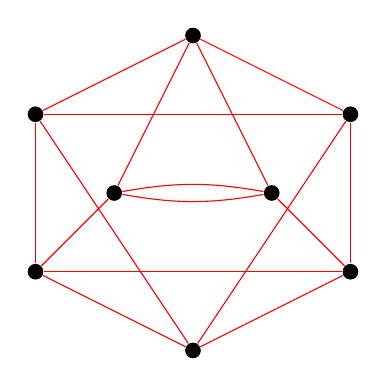
\begin{tikzpicture}
        \begin{scope}[every node/.style={fill,black,circle,inner sep=2pt}]
          \node at (0,0)  (1){};
          \node at (0,4) (20){};
          \node at (2,1)  (16z){};
          \node at (-2,1)  (81z){};
          \node at (-1,2) (77z){};
          \node at (1,2)  (20z){};
          \node at (-2,3)  (85z){};
          \node at (2,3)  (12z){};
        \end{scope}

        \begin{scope}[red]
          \path (1) edge (85z) edge (81z) edge (12z) edge (16z);
          \path (20) edge (85z) edge (77z) edge (20z) edge (12z);
          \path (81z) edge (85z) edge (77z) edge (16z);
          \path (85z) edge (12z);
          \path (12z) edge (16z);
          \path (16z) edge (20z);
          \path (20z) edge[bend right=10] (77z) edge[bend left=10] (77z);
        \end{scope}
      \end{tikzpicture}
      \small
      \emph{Figure:} $3$-isogeny graph on $\F_{97^2}$.
    \end{column}
  \end{columns}
\end{frame}

%%

\begin{frame}{Graphs lexicon}
  \begin{description}
  \item[Degree:] Number of (outgoing/ingoing) edges.
  \item[$k$-regular:] All vertices have degree $k$.
  \item[Connected:] There is a path between any two vertices.
  \item[Distance:] The length of the shortest path between two vertices.
  \item[Diameter:] The longest distance between two vertices.
  \item[$\lambda_1\ge\cdots\ge\lambda_n$:] The (ordered) eigenvalues
    of the adjacency matrix.
  \end{description}
\end{frame}

%%

\begin{frame}{Expander graphs}
  \begin{block}{Proposition}
    If $G$ is a $k$-regular graph, its largest and smallest
    eigenvalues satisfy
    \[k = \lambda_1 \ge \lambda_n \ge -k.\]
  \end{block}
  
  \begin{block}{Expander families}
    An infinite family of connected $k$-regular graphs on $n$ vertices
    is an \emph{expander family} if there exists an $\epsilon>0$ such
    that all \emph{non-trivial} eigenvalues satisfy
    $|\lambda| \le (1-\epsilon)k$ for $n$ large enough.
  \end{block}
  
  \begin{itemize}
  \item Expander graphs have \emph{short diameter} ($O(\log n)$);
  \item Random walks \emph{mix rapidly} (after $O(\log n)$ steps,
    the induced distribution on the vertices is close to uniform).
  \end{itemize}
\end{frame}

%%

\begin{frame}{Expander graphs from isogenies}
  \begin{block}{Theorem (Pizer)}
    Let $\ell$ be fixed. The family of graphs of \emph{supersingular}
    curves over $\F_{p^2}$ with $\ell$-isogenies, as $p\to\infty$, is
    an expander family\footnote{Even better, it has the Ramanujan
      property.}.
  \end{block}
  
  \begin{block}{Theorem (Jao, Miller, Venkatesan)}
    Let $\O\subset\Q(\sqrt{-D})$ be an order in a quadratic imaginary
    field. The graphs of all curves over $\F_q$ with \emph{complex
      multiplication by $\O$}, with isogenies of prime degree
    bounded\footnote{May contain traces of GRH.} by
    $(\log q)^{2+\delta}$, are expanders.
  \end{block}
\end{frame}

%%

\begin{frame}{Executive summary}
  \begin{itemize}
  \item Separable $ℓ$-isogeny = finite kernel = subgroup of $E[ℓ]$,
    \begin{itemize}
    \item eigenspace of $π$ iff $\F_q$-rational,
    \item distinct eigenvalues $λ≠μ$ define distinct directions on the
      crater.
    \end{itemize}
  \item Isogeny graphs have $j$-invariants for vertices and ``some''
    isogenies for edges.
  \item By varying the choices for the vertex and the isogeny set, we
    obtain graphs with different properties.
  \item $ℓ$-isogeny graphs of ordinary curves are volcanoes, (full)
    $ℓ$-isogeny graphs of supersingular curves are finite
    $(ℓ+1)$-regular.
  \item CM theory naturally leads to define graphs of horizontal
    isogenies (both in the ordinary and the supersingular case) that
    are isomorphic to Cayley graphs of class groups.
  \item CM graphs are expanders. Supersingular full $ℓ$-isogeny graphs
    are Ramanujan.
  \end{itemize}
\end{frame}

%%

\begin{frame}
  \centering
  \begin{tikzpicture}
    \begin{scope}[xscale=1.2,title]
      \def\crater{7}
      \foreach \i in {1,...,\crater} {
        \draw[fill] (360/\crater*\i:3cm) circle (5pt);
        \draw (360/\crater*\i : 3cm) -- (360/\crater*\i+360/\crater : 3cm);
        \foreach \j in {-1,1} {
          \draw[fill] (360/\crater*\i : 3cm) -- (360/\crater*\i + \j*360/\crater/4 : 4cm) circle (3pt);
          \foreach \k in {-1,0,1} {
            \draw[fill] (360/\crater*\i + \j*360/\crater/4 : 4cm) --
            (360/\crater*\i + + \j*360/\crater/4 + \k*360/\crater/6 : 4.5cm) circle (1pt);
          }
        }
      }
    \end{scope}
    
    \draw (0,1) node{\Huge\bf Thank you};
    \draw (0,-0.6) node{\large\url{https://defeo.lu/}};
    \draw (0,-1.3) node{\large\includegraphics[height=0.9em]{twitter.png}~\href{https://twitter.com/luca_defeo}{@luca\_defeo}};
  \end{tikzpicture}
\end{frame}

%%

\begin{frame}{Weil pairing}
  Let $(N,p)=1$, fix any basis \emph{$E[N]=〈R,S〉$}. For any points
  \emph{$P,Q∈E[N]$}
  \begin{align*}
    P &= aR + bS\\
    Q &= cR + dS
  \end{align*}
  the form \emph{$\det_N(P,Q) = \det\mat{a&b\\c&d} = ad - bc ∈ ℤ/Nℤ$}\\
  is \emph{bilinear}, non-degenerate, and independent from the choice
  of basis.

  \begin{block}{Theorem}
    Let $E/\F_q$ be a curve, there exists a Galois invariant bilinear
    map
    \[e_N: E[N] × E[N] → μ_N ⊂ \bar\F_q,\] \\
    called the \emph{Weil pairing of order $N$}, and a primitive
    $N$-th root of unity \emph{$ζ∈\bar\F_q$} such that
    \[e_N(P,Q) = ζ^{\det_N(P,Q)}.\] \\
    The degree \emph{$k$} of the smallest extension such that
    \emph{$ζ∈\F_{q^k}$} is called the \emph{embedding degree} of the
    pairing.
  \end{block}
\end{frame}

%%

\begin{frame}{Weil pairing and isogenies}
  \begin{block}{Note}
    The Weil pairing is Galois invariant $\;\;⇔\;\;\emph{\det(π|E[N]) = q}$.
  \end{block}

  \begin{block}{Theorem}
    Let \emph{$ϕ:E→E'$} be an isogeny and \emph{$\hat{ϕ}:E'→E$} its dual. \\
    Let \emph{$e_N$} be the Weil pairing of $E$ and \emph{$e_N'$} that
    of $E'$. %
    Then, for
    \[e_N(P,\hat{ϕ}(Q)) = e_N'(ϕ(P),Q),\]
    for any \emph{$P∈E[N]$} and \emph{$Q∈E'[N]$}.
  \end{block}
  
  \begin{block}{Corollary}
    \[e_N'(ϕ(P),ϕ(Q)) = e_N(P,Q)^{\deg ϕ}.\]
  \end{block}
\end{frame}

\end{document}


% LocalWords:  Isogeny abelian isogenies hyperelliptic supersingular Frobenius
% LocalWords:  isogenous


